\def\theTopic{Normal and t Distributions }
\def\dayNum{21 }

 \begin{center}
 {\bf {\large Theoretical Distributions}}
 \end{center}

  Whatever your field of study, you will need to read  research
  articles which present statistical inference like p-values and or
  confidence intervals.  We hope you now understand how those are
  properly used. In particular:
  \begin{itemize}
  \item Always report p-values. Smaller p-values provide stronger
    evidence against the null hypothesis.
  \item Confidence intervals are a list of ``plausible'' values.
    Our confidence is in the process used to build intervals, not
    in one interval. 
  \end{itemize}

  Many reports you read will refer to tests based on normal
  distributions rather than randomization and simulation.
  Before we had modern computers and the web apps we've been using,
  people had to use tables to look up probabilities to make confidence
  intervals and compute p-values.  We'll now look into these methods
  as a ``short cut'' alternative to simulations.
 % You've learned to use StatKey, and that's a useful skill because
 % it's freely available and you can actually use it to analyze real
 % data in the future.  However, if 
  We encourage you to take more statistics, for example regression 
  is a powerful technique used to describe relationships between
  quantitative variables.    We are happy to visit with you
  about possibilities for more statistics (Stat 217 is a great second
  course).  Part of the motivation for this lesson (and Unit 3 in
  general)  is to make it easier to
  continue your statistical adventures.

 
 \begin{center}
   {\Large\bf  Shapes of Data Distributions}
 \end{center}

  Look at these three different data sets:\\
\hspace*{2.6cm}A  \hspace*{5cm}B  \hspace*{4.5cm}C \\
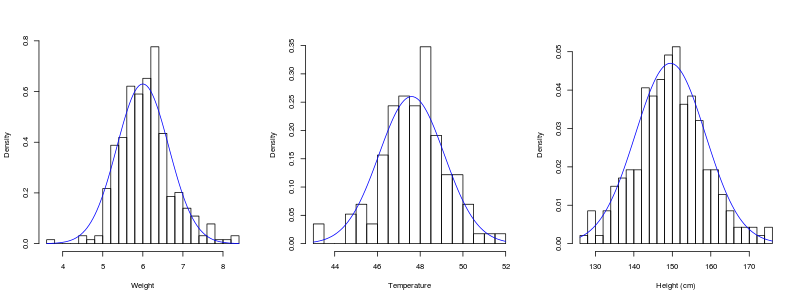
\includegraphics[width=.9\linewidth]{plots/normals.png}

A) Weights (g) of newly born lab rat pups. 
B) Mean annual temperatures ($^\circ F$) in Ann Arbor, Michigan.
C) Heights (cm) of 14 year old boys in Oxford, England. \vspace{-.1in}


\begin{enumerate}
  \item  In what way are these distributions similar and different?
\begin{students}
        \vspace{3cm}        
\end{students}

\begin{key}
{\it Means and spreads all differ, but the shapes are quite
  similar -- sort of bell-shaped. }
\end{key}

  Many distributions we look at have a shape similar to those above.
  Most of the data lies close to the mean, and the left and right
  sides are symmetric.  We call it ``bell-shaped'' and the best example is
  called the ``Normal'' distribution.
\end{enumerate}

Important fact:\\
{\sf Statistics vary from sample to sample, and the pattern is
  predictable.  For many statistics, the pattern of the sampling
  distribution resembles a normal distribution with a bell-shaped
  curve. }  Studying the normal distribution will allow us to find
probabilities for statistical inference which do not require running
simulations.

 {\bf Normal Distributions all have the same shape.\\
They differ only in mean ($\mu$) and spread ($\sigma$).}  We write $X
\sim N(\mu, \sigma)$ to say that random variable $X$ is normally
distributed with center $\mu$ and spread (officially: standard
deviation) $\sigma$.  This distribution
has two {\bf parameters}, $\mu$ and $\sigma$. 

{\bf Definition:  Random Variable} is a number which comes from some
random process, like randomly selecting one unit from a population and
measuring it.

The  {\bf Standard Normal Distribution} has center $\mu=0$ and spread
$\sigma = 1$.  We can ``standardize'' any normal distribution to make
it have center 0 and $\sigma = 1$ by subtracting $\mu$ and dividing by
$\sigma$. If a random measurement, $X$, has a N$(\mu, \sigma)$
distribution, then $Z = (X - \mu)/\sigma$ has a N(0,1) distribution. 
We use the standardized versions to say how many standard deviations
($\sigma$'s) an observation is from the mean ($\mu$). 


\begin{enumerate}
\setcounter{enumi}{1}
  \item  When you get back results from standardized tests, they give
    a score and tell you your ``percentile rank'', the percentage
    of test takers who score at your level or below.  The exam scores have
    an approximately normal distribution.  For example, with ACT, $\mu
    = 21$ and $\sigma = 5$.
    \begin{enumerate}
    \item What is the standardized $z$ score for Amber who got 27 on the ACT?
\begin{students}
        \vspace{2cm}        
\end{students}
\begin{key}
  $$ \frac{25 - 21}{5} = 1.20$$
\end{key}
    \item What is Amber's percentile rank?  Plug her standardized score into the
      first line of this web app 
      \url{http://shiny.math.montana.edu/prob} and select
      \fbox{Lower}. (Leave the last box set to \fbox{Normal}
      distribution.) Explain what the number means in terms of other
      test takers.  
\begin{students}
        \vspace{1cm}        
\end{students}

\begin{key}
 {\it .885 or 88.5\% of students taking the ACT are at this level or lower.}
\end{key}
   \item Bert took the SAT instead of the ACT, and
      SAT scores are normally distributed with mean $\mu = 1500$
     and spread $\sigma = 300$. Bert's score was  1720. What is Bert's
     standardized score?
\begin{students}
        \vspace{2cm}        
\end{students}
\begin{key}
  $$ z = \frac{1720 - 1500}{300} = 0.733$$
\end{key}
    \item What is Bert's percentile rank? Compare how well he did on
      the SAT with how well Amber did on the ACT. 
\begin{students}
        \vspace{2cm}        
\end{students}

\begin{key}
 {\it .768 or 78.8\% of students taking the SAT are at this level
    or lower.  Amber did better relative to others taking the ACT than
    Bert did relative to SAT takers.}
\end{key} 
  \end{enumerate}
\end{enumerate}

{\bf Definition:  Probability}: the proportion of times -- in the long run
-- that a particular outcome occurs.  For example, the probability of
drawing a ``heart'' from a well-shuffled deck of cards is
0.25. Probabilities must be between 0 and 1. 


\begin{minipage}{.80\linewidth}
{\bf Normal Probabilities} are areas under the normal curve.  Area
under the  entire curve is 1.   What area is shaded for this normal
distribution? \vspace*{2cm}
\end{minipage}
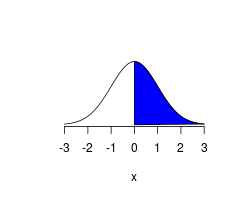
\includegraphics[width=.2\linewidth]{plots/halfNormal.png}
\vspace{-1.9cm}

We can also go from a percent to a percentile (or, from a probability
between 0 and 1 to a {\bf quantile}) by back--solving the ``Z'' formula for
$X$ like this:  
$$\mbox{Start with } Z = \frac{X-\mu}{\sigma}  \mbox{ and solve for
  $X$ to get }
  X = Z\sigma + \mu $$

What SAT score is needed to be in the top 10\% of SAT takers?\\
In the same web app, put 0.10 in the second box and click upper (or 0.90
and click lower). That returns a $Z$ value of 1.282, so 
$ X = 1.282 \times 300 + 1500 = 1884.5$.  SAT  scores are always
multiples of ten, so a score of 1890 puts a person into the top 10\%,
or above the 90$^{th}$ percentile. 

\begin{enumerate}
\setcounter{enumi}{2}
\item {\bf Your Turn:} Suppose birth weights of full term babies have
  a $N(3000, 700)$ (in grams) distribution. Show your work, that is,
  how you standardize each value, or ``unstandardize'' to get a
  percentile.
\begin{enumerate}
\item 
  How heavy is a baby whose weight is at the  98$^{th}$
  percentile? The 5$^{th}$ percentile? 
\begin{students}
        \vspace{1cm}        
\end{students}

\begin{key}
{\it Standardized percentiles are 2.054 and -1.645.  Converting to
    birth 
    weights( times 700 + 3000): 4438g and 1848.6g. }
\end{key}

\item What is the probability that a randomly chosen baby will weigh
  under 3500g?  Under 2500g?
\begin{students}
        \vspace{1cm}        
\end{students}

\begin{key}
 {\it $Z = \pm 500/700 = \pm 0.714$, Probabilities: 0.762, 0.237}
\end{key}
\item What proportion of birth weights are within one standard deviation of the  mean? Within 2 SD's? within 3 SD's?
\begin{students}
        \vspace{.5cm}        
\end{students}

\begin{key}
 {\it 0.683, 0.955, 0.997 }
\end{key}

  \end{enumerate}
\end{enumerate}

Note: The last question gives us a useful rule of thumb which we call
the empirical rule.  The middle value (probability of being within
2 SD's) is usually rounded to 95\%.
\begin{students}

\end{students}

\begin{center}
  {\Large\bf t Distributions}
\end{center}

To standardize a normal distribution,  we need to know its true mean,
$\mu$, true standard deviation, $\sigma$. Problem: we never know the
true parameter values.  We can work around the unknown
mean pretty easily, but not knowing $\sigma$ causes a bit of a problem.

{\bf Discuss}: Look back to Activity 2 notes (p 13-14) and estimates of spread. What can we plug in to estimate the unknown population spread,
$\sigma$? 
\begin{students}
        \vspace{2cm}        
\end{students}

\begin{key}
 {\it $s$, the spread in the sample}
\end{key}

In the early 1900's, Mr.~Gossett was working for Guinness Brewery.  He
discovered that using an estimated instead of ``known'' $\sigma$
changes the distribution from regular normal to something called a
$t$-distribution which is more spread out.  Furthermore, there is not
just one $t$-distribution, but many depending on your sample size.

This make sense because as sample size gets big, $s$ becomes a better
and better estimate of $\sigma$.  Here is a picture of several
t-distributions compared to a standard normal distribution.  

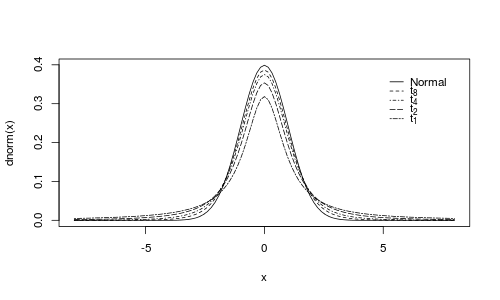
\includegraphics[width=.7\linewidth]{plots/t-normalDensities.png}
 % curve(from=-8,to=8, dnorm(x))
 % curve(from=-8,to=8, dt(x,1) , lty=6, add=TRUE)
 % curve(from=-8,to=8, dt(x,2) , lty=5, add=TRUE)
 % curve(from=-8,to=8, dt(x,4) , lty=4, add=TRUE)
 % curve(from=-8,to=8, dt(x,8) , lty=2, add=TRUE)
 % legend(5, .38, bty="n", lty=c(1,2,4,5,6), c("Normal",expression(t[8]),expression(t[4]),expression(t[2]),expression(t[1])))
 %  dev.copy(png,"plots/t-normalDensities.png",
 %  height=300,width=500);dev.off()

We can standardize like this:
$$ t = \frac{X - \xb}{s}\mbox{\ \  or go the other way:\ \ } x = \xb
+ t^* \times s$$
and use the same web app to compute the 
probabilities and quantiles for $t$-distributions just as we did with normal
distributions. The one additional fact needed is that for a one-sample
mean, we use $n-1$ (sample size minus 1) as the {\bf``degrees of
  freedom''} which define the t distribution needed.  When you select
\fbox{t} instead of \fbox{normal} distribution, you'll be able to set
the degrees of freedom.

Example:\\
Heights for adult men in the US are close to normally distributed.
We'll take 70 inches to be the mean height. From a simple random
sample of 20 men,  we compute a sample standard deviation of $s = 3.3$
inches.  
\begin{enumerate}
\setcounter{enumi}{5}
\item You will use a t-distribution with what degrees of freedom?
\begin{students}
        \vspace{1cm}        
\end{students}

\begin{key}
 {\it 19}
\end{key}

\item Use the appropriate $t$ distribution to determine how unusual it
  is to see a man who is over 76 inches tall. Show your standardized
  value and the probability.
\begin{students}
        \vspace{1cm}        
\end{students}

\begin{key}
 {\it t = 1.818, $P(t_{19} > 2) = 0.042$ }
\end{key}

\item Under 68 inches tall?
\begin{students}
        \vspace{1cm}        
\end{students}

\begin{key}
{\it  t = -1.212, $P(t_{19} < -1.212) = 0.12$ }
\end{key}

\item Between 65 inches and 75 inches? (You have to enter each
  standardized value, selecting ``Lower'', and subtract to get the
  area in between.)
\begin{students}
        \vspace{1cm}        
\end{students}

\begin{key}
 {\it $t$ values are 1.515 and -1.515. subtract 0.073 from 0.927,
    or use the \fbox{Center} choice to get 0.854. }
\end{key}

\end{enumerate}


\begin{center}
  {\large\bf Take Home Message}
\end{center}
 
\begin{itemize}
\item Theoretical distributions are a shortcut method to obtain
  probabilities.
\item Normal and t distribution probabilities are areas under a
  curve. We can get them from statistical computer packages.
\item Both normal and t distributions are symmetric and
  bell--shaped. The t-distributions are more spread out because we
  have to estimate the standard deviation.
\item When $\sigma$ is known use a normal distribution. Otherwise, use
  a t-distribution with $n-1$ degrees of freedom for just one
  sample. (This changes for 2 or more samples).
\item To look up normal or t probabilities, we have to standardize by
  subtracting $\mu$ and dividing by $\sigma$ (for normal) or $s$ (for
  t). The standardized score tells us how many standard deviations we
  are from the center.
\item You need to be able to go either way: find a probability from a
  Z or t score, or find the percentile from the probability.
\item Empirical Rule for data with a normal distribution:\\
  \begin{itemize}
  \item 68\% of the values fall within one SD of the mean.
  \item 95\% of the values fall within 2 SD of the mean, and 
  \item 99.7\% of the data fall within 3 SD of the mean.
  \end{itemize}
\end{itemize}


%% 5 pages.  Add CLT or LLN?

 % x<- c(0,seq(0,3,.01))
 % y<- c(0,dnorm(x[-1]))
 % curve(dnorm(x), from = -3, 3, yaxt="n", ylab="", bty="n")
 % polygon(x,y,col="blue")
 % dev.copy(png,file="halfNormal.png", height=200,width=240);dev.off()

%% 5 pages.  Add CLT or LLN?

